
%\section{Datasets}

The example analysis studied here involves a so-called Daltiz-plot analysis.  In such analyses, the distribution of events in a 2-D space is typically fit to extract some information of physical interest.  The regions of the Daltiz-plot that tend to have the highest sensitivity to the desired information are the {\em edges}.  Unfortunately, the edge regions also typically have the most background contamination and the least discrimination against background.  Therefore, traditional classifier-based selections tend to produce selections for Dalitz-plot analyses with lower efficiency near the edges.   

This study uses simulated event samples produced using the official LHCb simulation framework.
The software used for the generation of the events is described in LHCb publications as follows :

\begin{quote}
In the simulation, $pp$ collisions are generated using
PYTHIA~\cite{Sjostrand:2006za} 
with a specific LHCb configuration~\cite{LHCb-PROC-2010-056}.  Decays of hadronic particles
are described by EvtGen~\cite{Lange:2001uf}, in which final state
radiation is generated using PHOTOS~\cite{Golonka:2005pn}. The
interaction of the generated particles with the detector and its
response are implemented using the GEANT
toolkit~\cite{Allison:2006ve, Agostinelli:2002hh} as described in
Ref.~\cite{LHCb-PROC-2011-006}.
\end{quote}

All simulated event samples are generated inside the LHCb detector acceptance.
The signal used in this analysis consists of $D_s^\pm\to\pi^+\pi^-\pi^\pm$ decays, simulated
using the $\textrm{D}\_\textrm{DALITZ}$ model of EvtGen to simulate the intermediate resonances which contribute to the
three pion final state. The background candidates are three pion combinations reconstructed in
simulated samples of $c\bar{c}$ and $b\bar{b}$ events, where the charm and bottom quark decays are
inclusively modelled by EvtGen. The simulated events contain ``truth'' information which identifies them as
signal or background, and which identifies the physical origin of the three pion combinations reconstructed
in the $c\bar{c}$ and $b\bar{b}$ simulated samples.

\begin{figure}[] 
  \centering 
  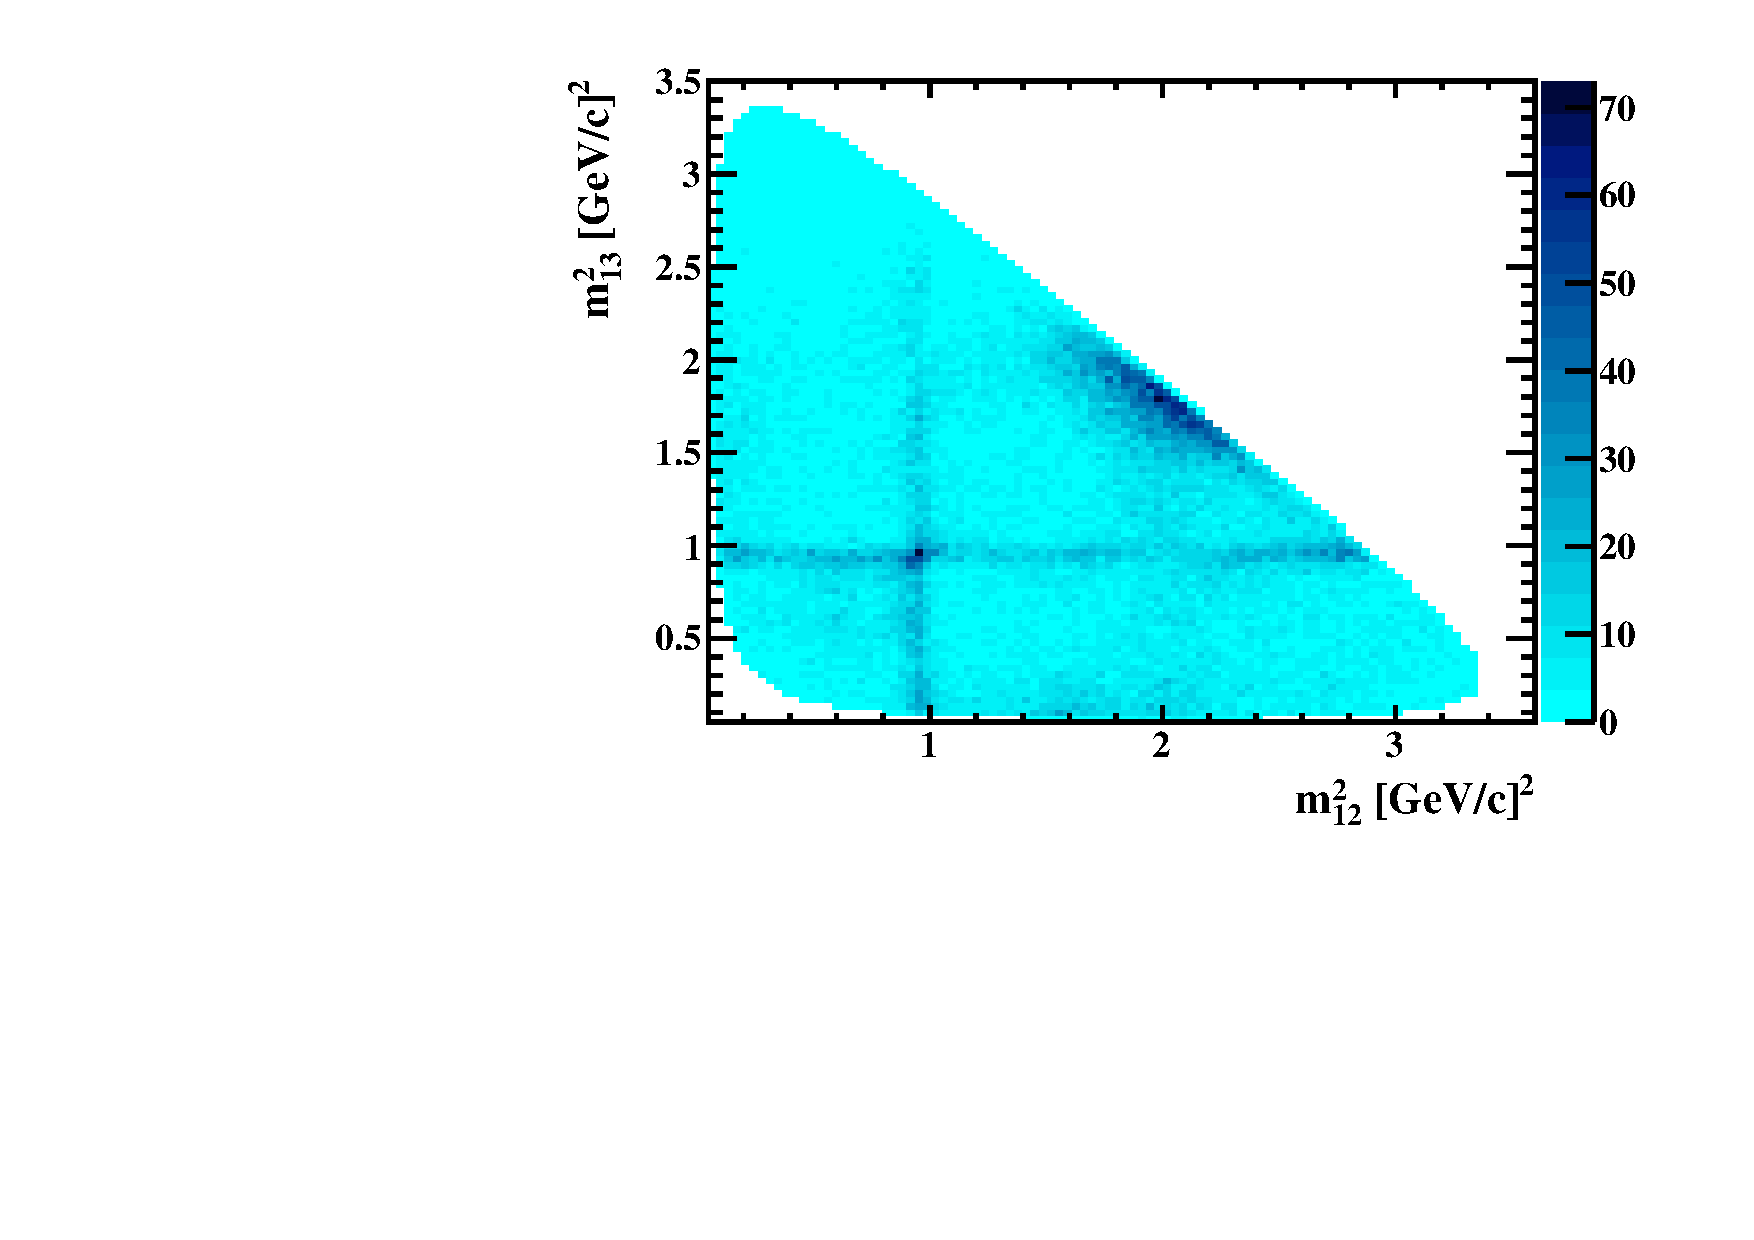
\includegraphics[width=0.49\textwidth]{DP_sig.pdf}
  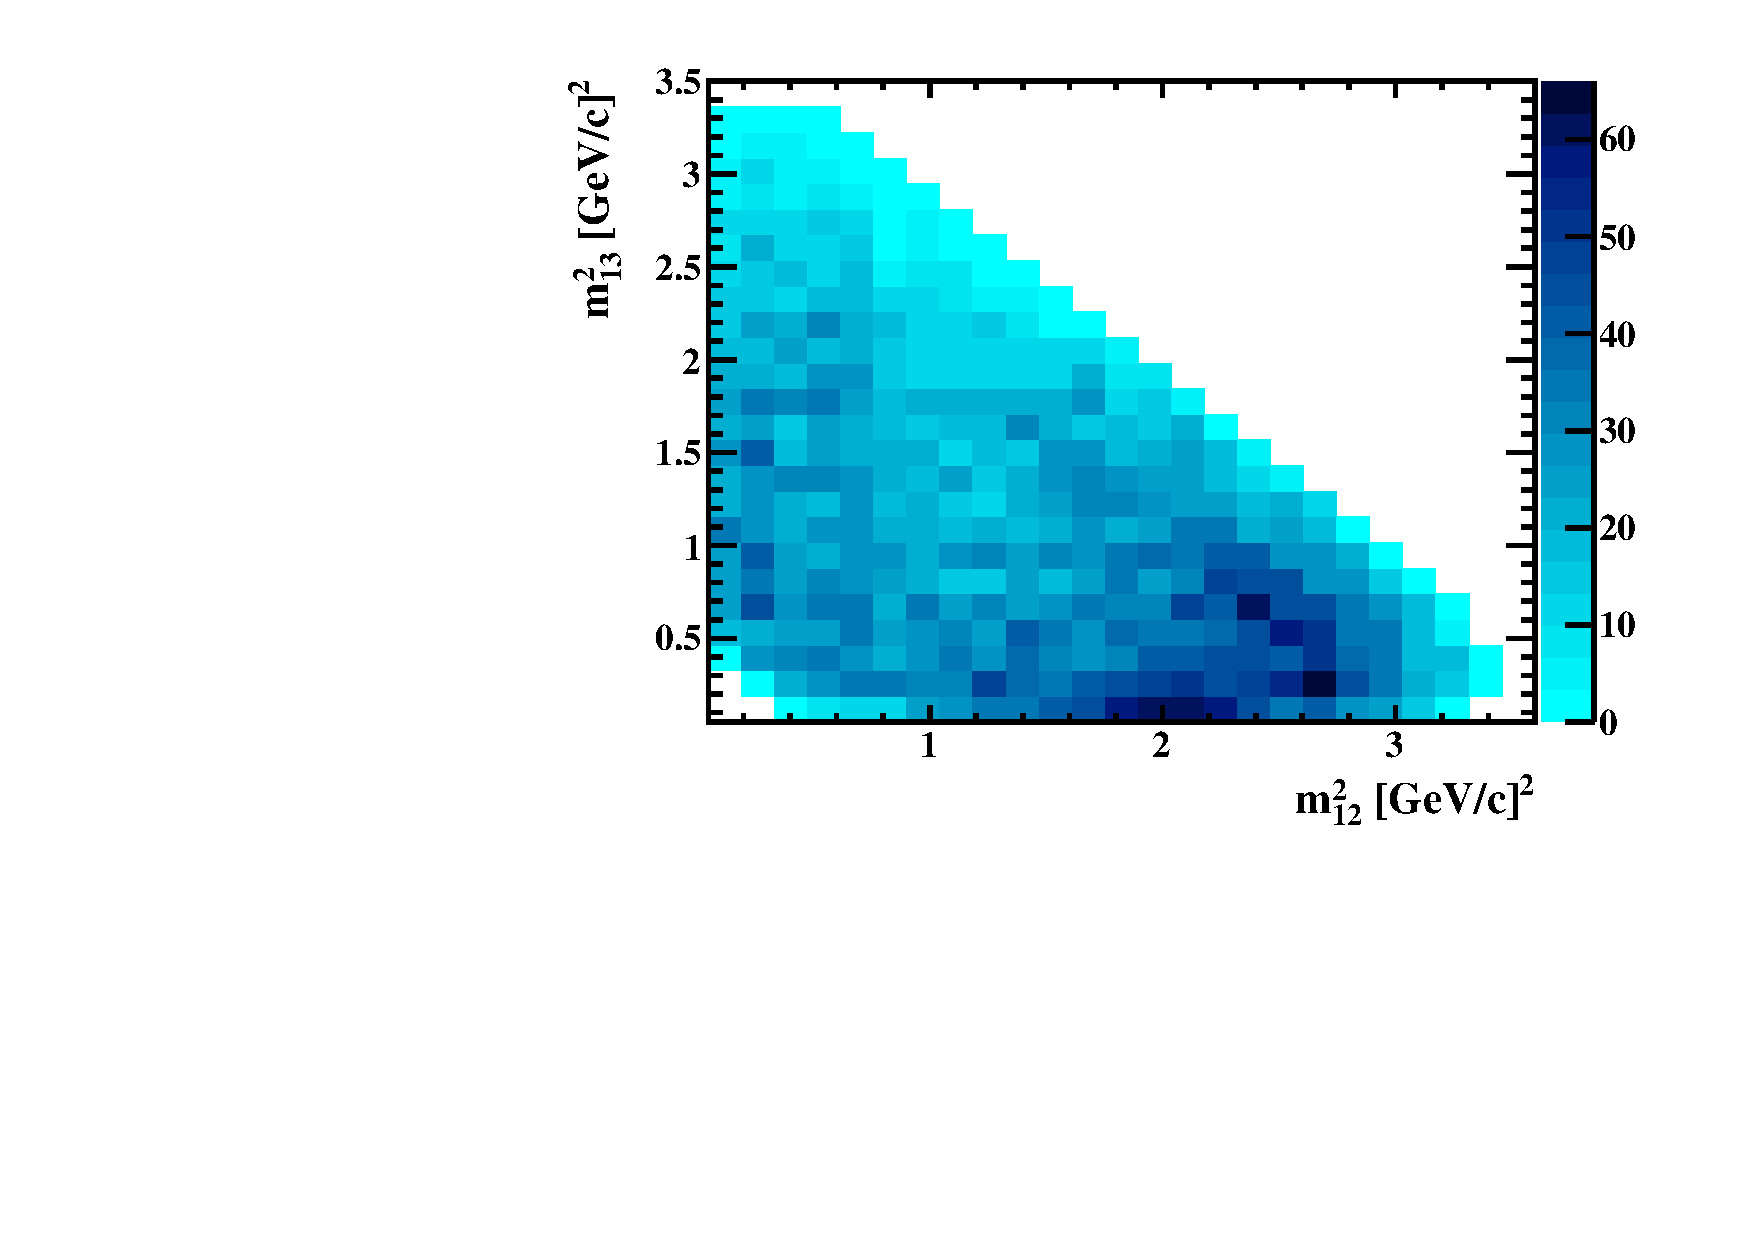
\includegraphics[width=0.49\textwidth]{DP_bkgd.pdf}
  \caption{\label{fig:dalitz} Dalitz-plot distributions for (left) signal and (right) background for the $D_s^\pm\to\pi^+\pi^-\pi^\pm$.  The three pions are labeled here as 1, 2 and 3.}
\end{figure}

Figure~\ref{fig:dalitz} shows the Dalitz-plot distributions for signal and background events.  These samples are split into training and testing samples and then various BDTs are trained.  For the BDTs designed to produce uniform selections, the $\vec{y}$ variates are the Dalitz masses with the choice of uniform selection efficiency on signal candidates in the Dalitz-plot.  
Figure~\ref{fig:dalitz_rocs} shows the ROC curves obtained for the various classifiers studied in this paper.  For the UGBFL algorithms, there is a choice to be made for the value $\alpha$ which defines the relative weight of the flatness loss {\em vs} AdaLoss.  As expected, increasing $\alpha$, which increases the weight of AdaLoss, drives the ROC curve to be similar to AdaBoost.  Analysts will need to choose how much ROC performance to sacrifice to gain uniformity in the selection efficiency.  In general, the ROC curves for the uniform-driven BDTs are not too different from AdaBoost.  



\begin{figure}[] 
  \centering 
  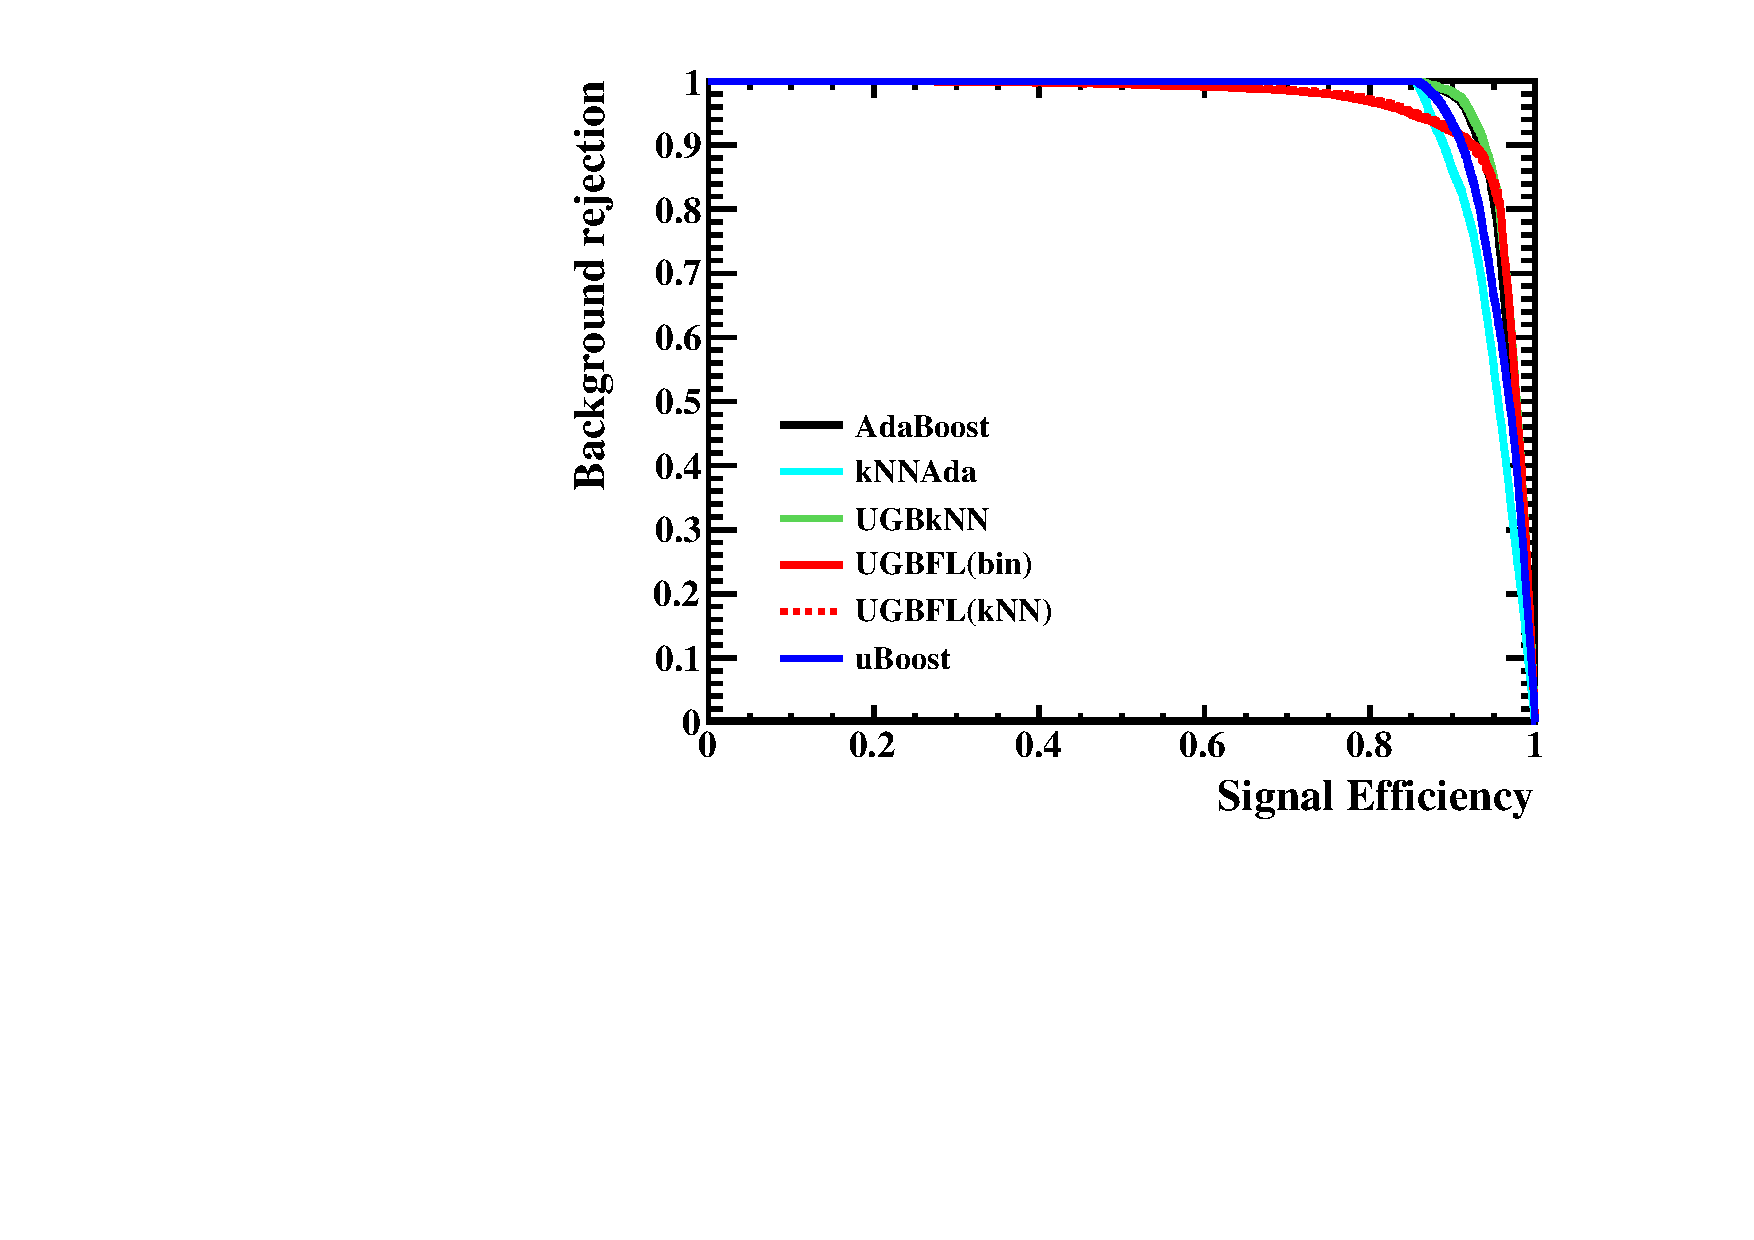
\includegraphics[width=0.49\textwidth]{ROC_DP.pdf}
  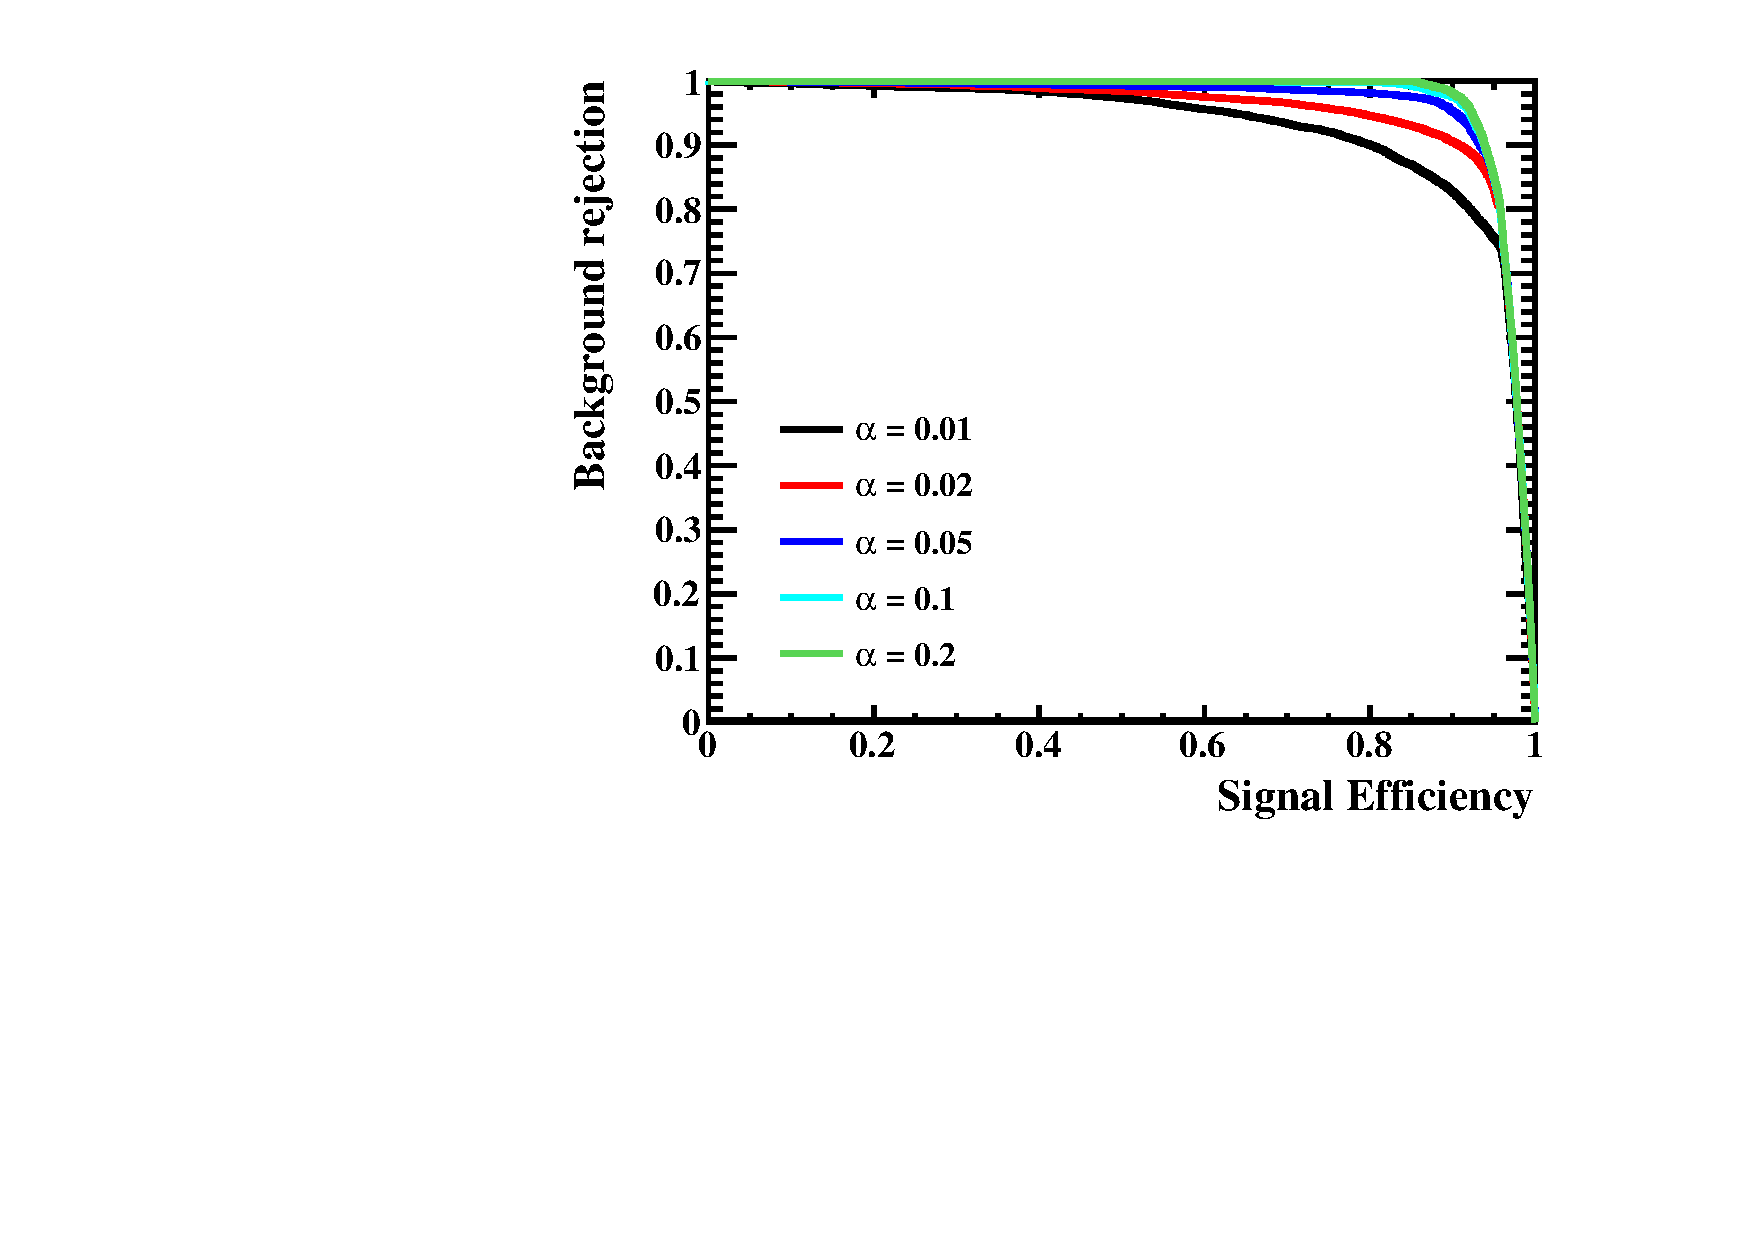
\includegraphics[width=0.49\textwidth]{ROC_DP_Alpha.pdf}
  \caption{\label{fig:dalitz_rocs} (left) ROC curves for classifier algorithms studied in this paper.  (right) ROC curves for UGBFL(bin) for differnet values of $\alpha$.}
\end{figure}

Figure~\ref{fig:dalitz_results} shows the efficiency obtained for each classifier {\em vs} distance from the a corner of the Dalitz-plot\footnote{The Dalitz-plot is essentially a triangle with three corners. Our defnition of this distance is ${\rm MIN}\left[(m(D_s)-m(\pi))^2 - m_{ij}^2\right]$, where $ij$ is 12, 13 and 23.}.  The AdaBoost algorithm, as expected, produces a much lower efficiency in the interesting corner regions.  The kNNAdaBoost algorithm does not improve upon the AdaBoost result much.  This is likely due to the fact that while kNNAdaBoost uses non-local kNN information, it does not utilize global information.
The UGBFL (binned and unbinned kNN) and uBoost algorithms each produce an efficiency which is statistically consistent with uniform across the Dalitz plot.  
As stated above, the analyst is free to optimize the choice of $\alpha$ for UGBFL by defining a metric that involves signal efficiency, background rejection and uniformity, {\em e.g.}, using uniformity metrics discussed in detail in Appendix~A.  

\begin{figure}[] 
  \centering 
  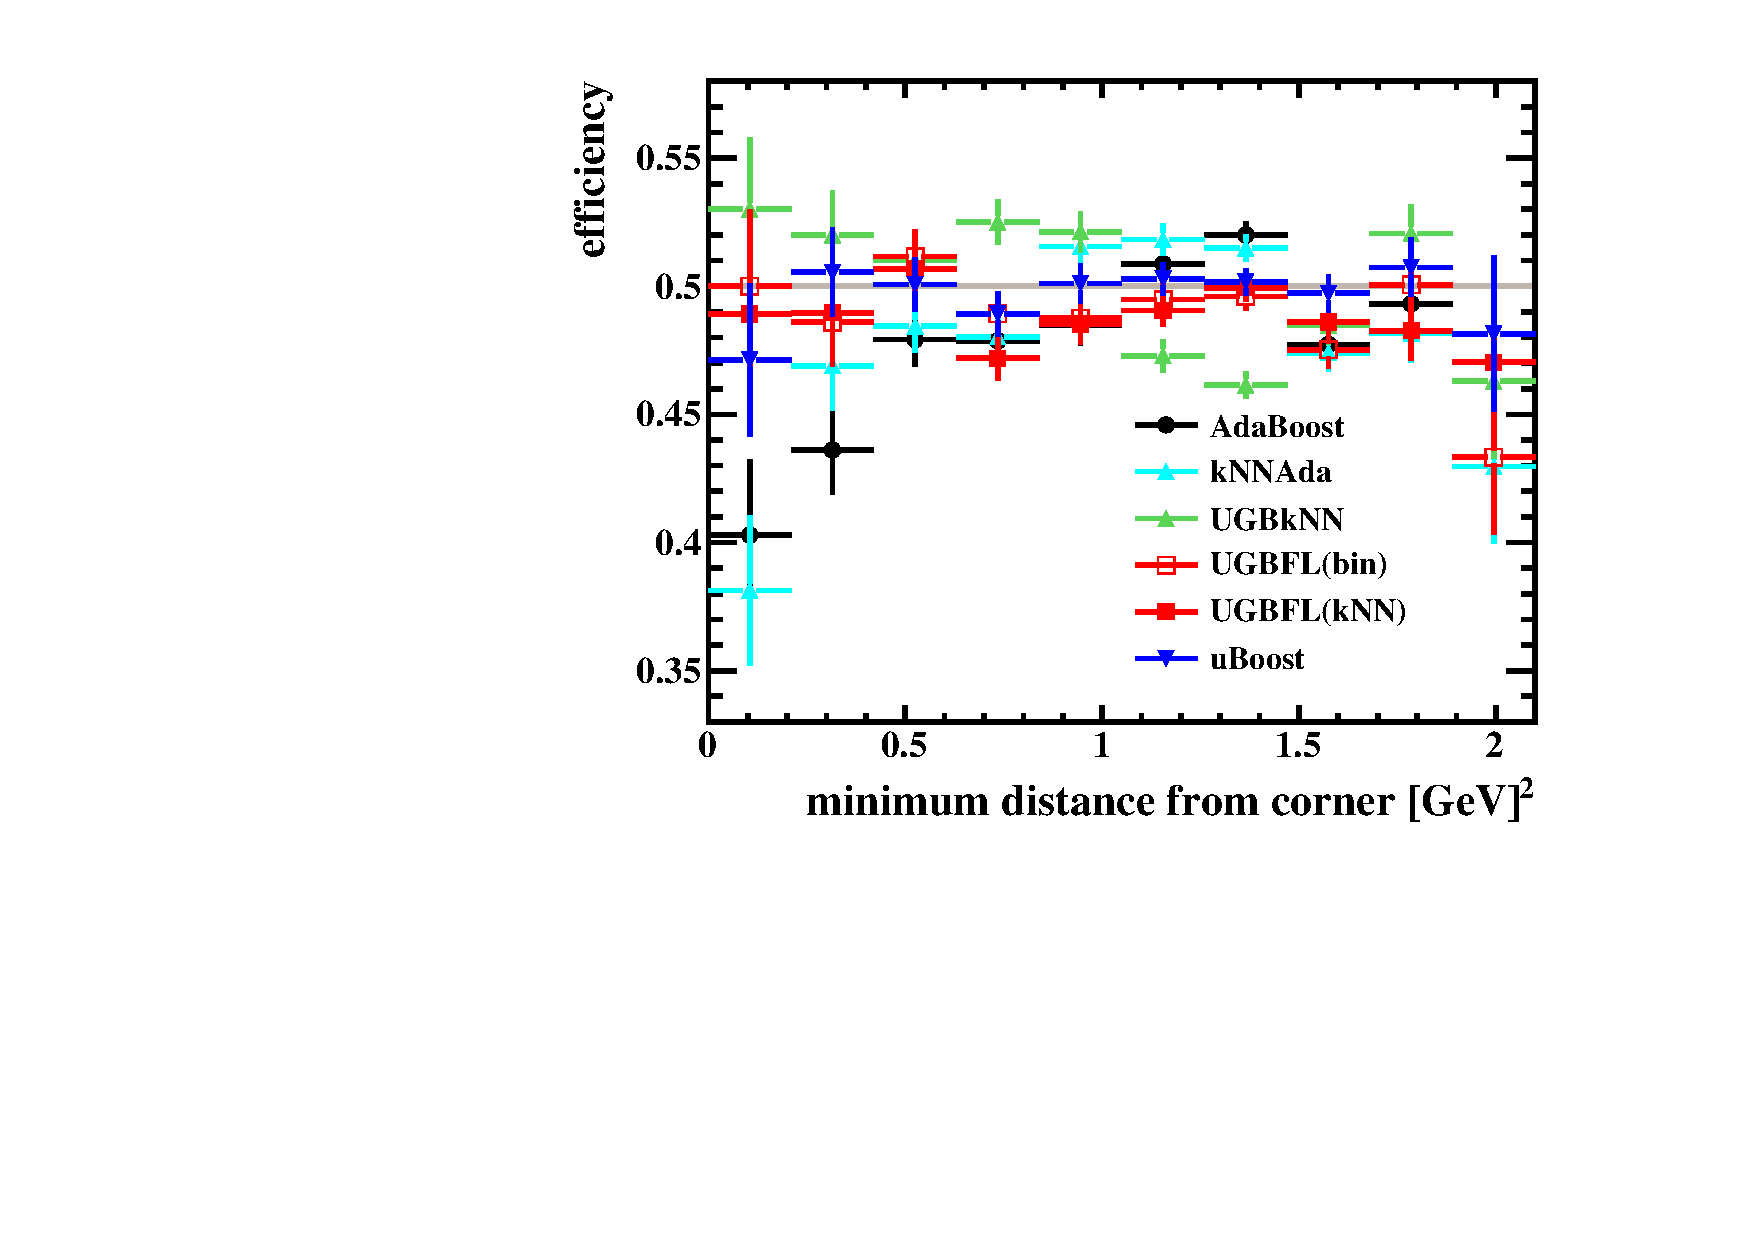
\includegraphics[width=0.49\textwidth]{DP_compare.pdf}
  \caption{\label{fig:dalitz_results} Efficiency {\em vs} distance to a corner of the Dalitz-plot.  An arbitrary working point of 50\% integrated efficiency is displayed.}
\end{figure}


As a separate study using the same data samples, consider the case where one has simulated signal events and uses data from a {\em nearby} region, a so-called sideband, for background.  This is a common situation in particle-physics analyses.  Figure~\ref{fig:md_results} shows the training samples used.  A major problem can arise in these situations as typically input variates to the BDT are correlated with the parent particle mass.  Therefore, the BDT may learn to reject the background in the training using the fact that the mass of the background and signal candidates is different.  This is just an artifact of how the background sample is obtained and will not be true for background candidates {\em under} the signal peak.  Figure~\ref{fig:md_results} shows the background mis-indentifcation rate {\em vs} $D$ candidate mass.  AdaBoost has clearly learned to use this mis-match in signal and background candidate masses in the training.   The background in the region of the signal is about three times higher than one would expect from looking only at the sideband data.  


\begin{figure}[] 
  \centering 
  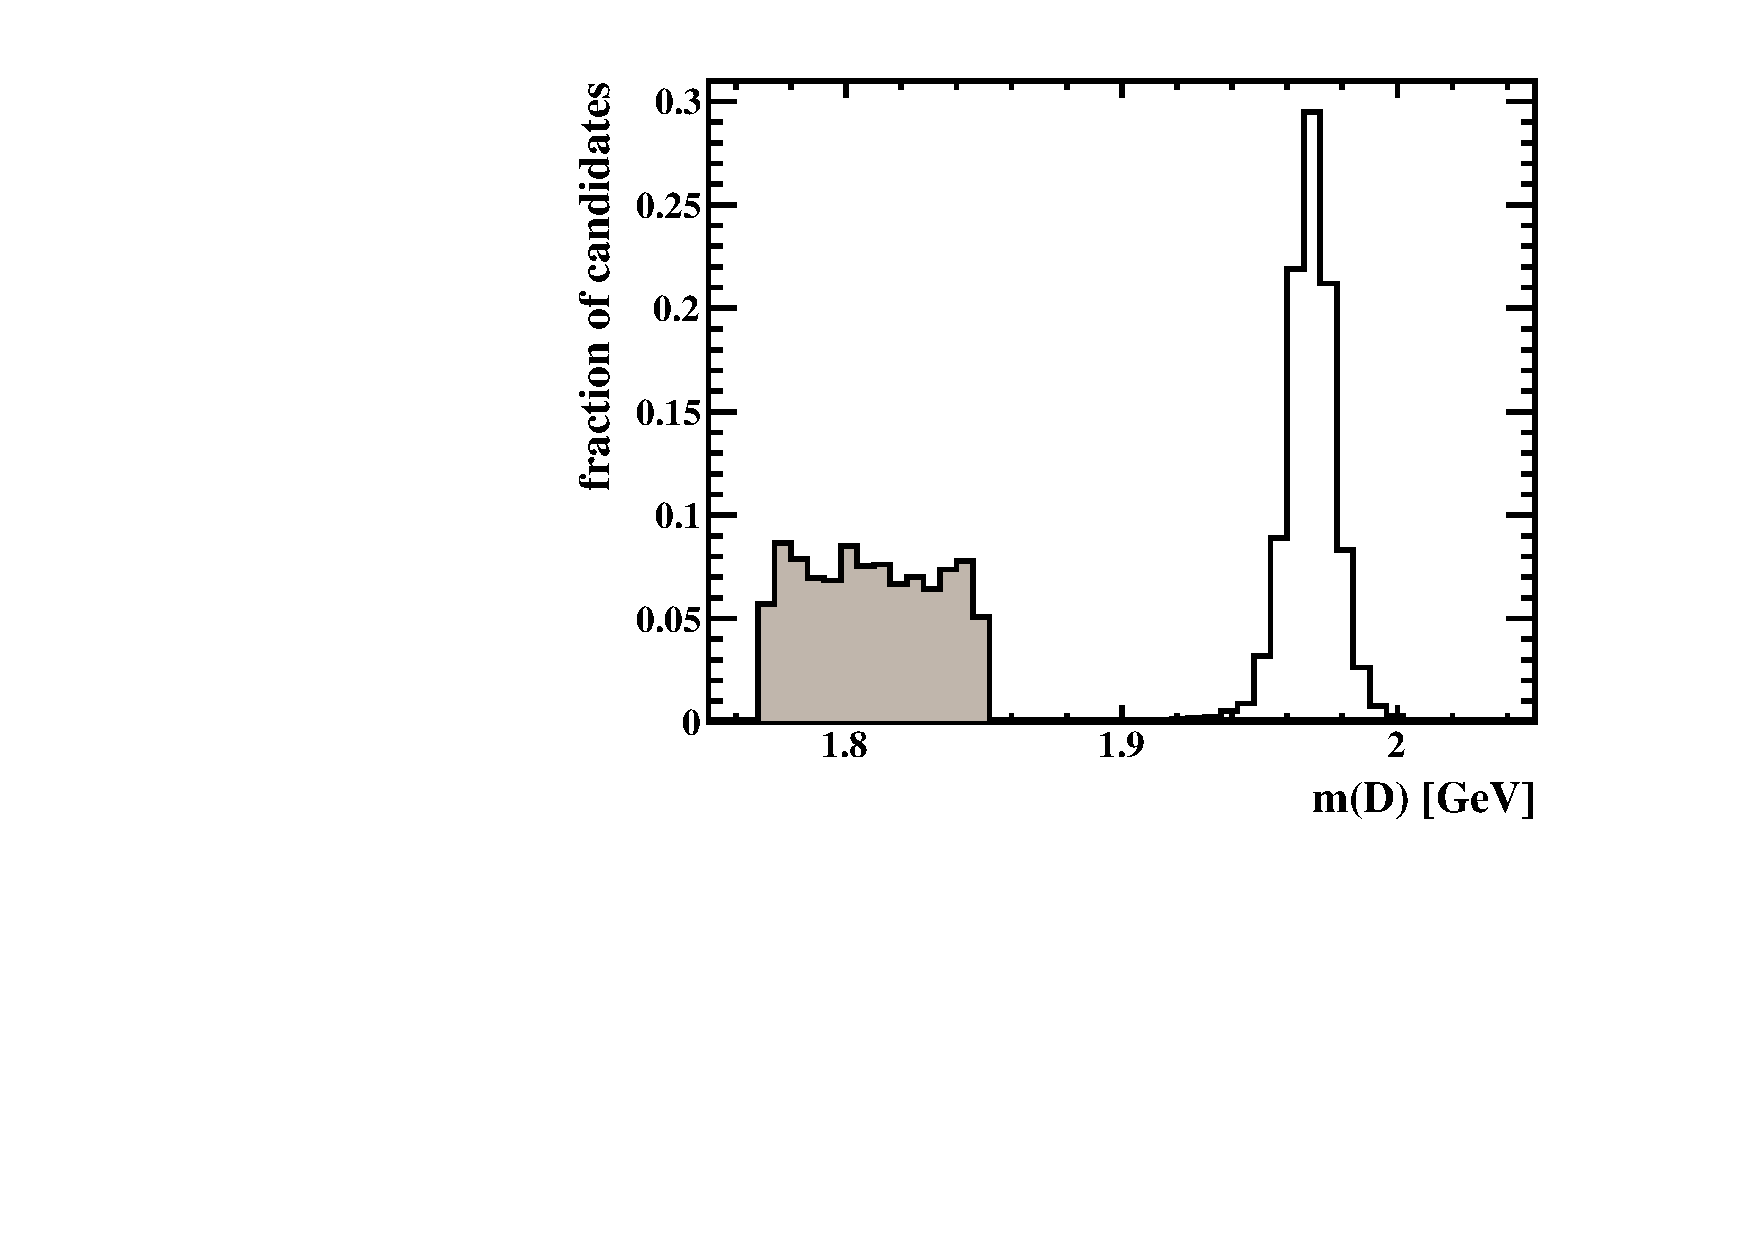
\includegraphics[width=0.49\textwidth]{mD_train.pdf}
  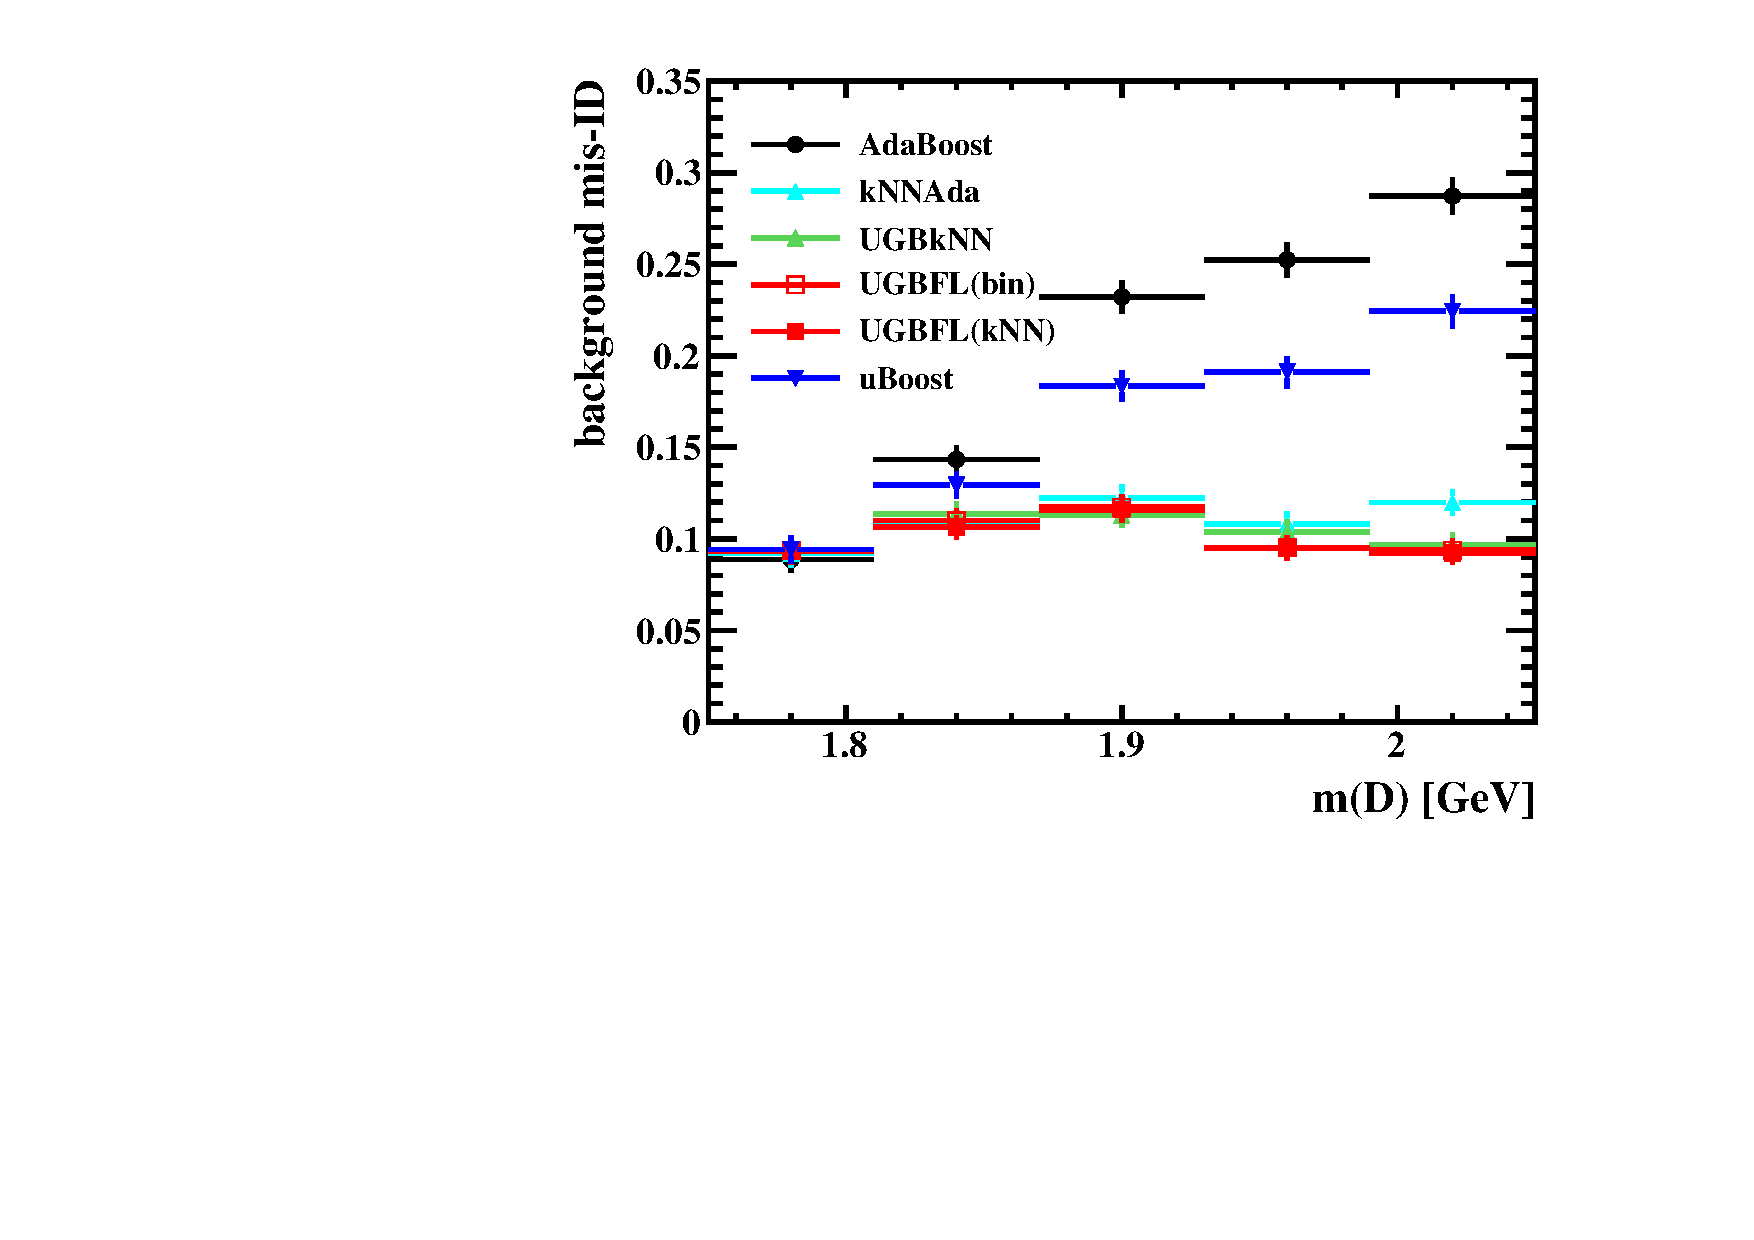
\includegraphics[width=0.49\textwidth]{MD_eff.pdf}
  \caption{\label{fig:md_results} (left) Signal and (filled) background samples used in training.  (right) Background mis-identification {\em vs} $D$ candidate mass for an arbitrary working point of 10\% background mis-identification in the training region $1.75 < m(D) < 1.85$~GeV is displayed.}
\end{figure}

Figure~\ref{fig:md_results} also shows the background mis-indentifcation rate {\em vs} $D$ candidate mass for the various uniform classifiers where $y = m(D)$ and the choice is for uniformity in the background efficiency\footnote{The algorithms in this paper can easily be made uniform on signal, background or both.}.  
The uBoost algorithm does better than AdaBoost here but is still not optimal.  The way that uBoost achieves uniformity is not such that it can be trusted to work outside the region of training.  The algorithms presented in this paper each does well in achieving similar performance in the training and signal regions.  
Consider, {\em e.g.}, the UGBFL approach to achieving uniform selection efficiency.  In this case the training drives the BDT response itself to have the same PDF everywhere in the region $1.75 < m(D) < 1.85$~GeV (the training region).  
This does not gaurantee that the BDT response is truly independent of $m(D)$ outside the training region, but does strongly suppress learning to use $m(D)$ and in this example results in the desired behavior.  
Finally, if both high and low $m(D)$ sidebands had been used, it is possible for a BDT to create a fake peak near the signal peak location.  The use of UGBFL greatly reduces the chances and possible size of such an effect.


